%\documentclass{article}
\documentclass[letterpaper, 10 pt, conference]{ieeeconf}
\usepackage[utf8]{inputenc}
\usepackage{url}
\usepackage{hyperref}
%\usepackage[showframe=true]{geometry}
%\usepackage[usenames,table]{xcolor}
%\usepackage{titlepic} 
\usepackage{graphicx}
\usepackage{subfigure}
\usepackage[font=small]{caption}
\usepackage{amssymb,amsmath,amsthm}
\usepackage{capt-of}
\usepackage{textcomp}
%\usepackage{caption}
%\usepackage{titling}
\usepackage{algorithm2e}
\usepackage{amsmath,lipsum}

%\overrideIEEEmargins

\title{
\includegraphics[scale = 0.05]{img/logo_unige.jpeg} \\ Energy saving room scheduling system for smart hotels}
\author{Ernesto Denicia, Emanuele Sansebastiano, Rocco Caravelli}
%\date{July 2016}

% geometry and page settings
%\geometry{includehead,includefoot}
%\geometry{inner=2cm,outer=2cm,top=2cm,bottom=2cm}
\parskip = 3pt
\parindent = 0pt
%\\ make a blannk line where they r located

\newcommand\T{\rule{0pt}{2.6ex}}% aggiungi spazio sopra riga di tabella

\DeclareMathOperator{\Ker}{Ker}
\DeclareMathOperator{\spn}{span}
\DeclareMathOperator{\sinc}{sinc}

% links colors
\hypersetup{
	colorlinks,
%	linkcolor={orange},
%	citecolor={black},
%	urlcolor={blue}
}



\begin{document}		
%	\hspace{\stretch{1}}
%	\begin{minipage}{0.25\linewidth}
%	\centering
%	\end{minipage}\hspace{\stretch{1}}
%	
%	\begin{minipage}{0.50\linewidth}
%		\centering
%		\maketitle
%	\end{minipage}\hspace{\stretch{1}}
%
%	\begin{minipage}{0.25\linewidth}
%	\centering
%	\end{minipage}\hspace{\stretch{1}}

%
\includegraphics[scale=0.1]{img/unige_sys.jpg}
\maketitle

\small

\section{Abstract}
The energy consumption is probably the most important aspects engineers have to take into account when they project a robot case or plan the action sequence to make it do. Generally, this problem is handle by optimal path research and optimal decision analysis. There are infinitive application in robotics regarding optimal storage strategy, for instance, manipulators managing storehouse have to decide where they have to store the packs according to shortest time spend, force and velocity they can apply on the pack (fragile or not), and best storage location according to the specifics of the object: the robot do have to put milk in a fridge, not in a hoover. Our analysis deals with this last case: where I do have to put something which must stay in specific temperature bounds. In particular, we analysed how the customers are placed in hotel room according to their needs, at first, the maximal revenue the hotel owner can get and the minimal energy usage to keep the temperature feasible to live by law. In this paper we are going to analyse the Winter period, but the identical approach can be used to find the optimal distribution during Summer.

\section{Introduction and proposal}
This paper deals with the necessity of reducing the energy loss in hotels related to the usage of heat sources (radiators, heat pumps, etc..).
Since a hotel has to provide a fixed minimum in every room used to host of 20 $\pm$ 2 \textcelsius \ by the norm DPR n° 412/1993, during Winter, at least in Europe, hotel managers need to turn on heaters. Assuming the buildings we are observing have the possibility to turn on and off the heat sources of each room independently from the other ones we wonder if the usage of the heat source is just dependent on the dimension of the specific room or if the other rooms will contributes to reduce the energy required to heat up the considered room. Moreover, we assume that if none booked a room on a day, that heater is not active in that room on that specific day. In order to see check it we made a lumped parameter model of the hotel using a on/off controller, having heat pumps as heating (and cooling) system source. These heat pumps directly blow wormed air in the room (forced convection), so they are very fast, and easy to control by an on/off control. The figure \ref{figTemper_onoff} shows that, thanks to the fact the room located on the first floor (blue line) is occupied on the days 2, 4, 5 and the room located on the third floor (blue line) is occupied on the days 2, 4, 6, the room located on the second floor (red line), which is in the middle, receives a consistent heat flux from the other two. That room is never booked on the mentioned period, but its temperature is almost always above to minimum temperature required to keep the heat pump off (18.5 \textcelsius).
Finally, we have the proof the temperature of a room influences the one of the other and vice verse. Thus, we want to formulate and optimal decision algorithm, which takes in consideration all the rooms in their complexity, to accept, at first, the best requests combination among the ones we have, and then, optimize the distribution of the accepted costumers in the rooms available. 

\begin{figure}[htbp]
	\centering
	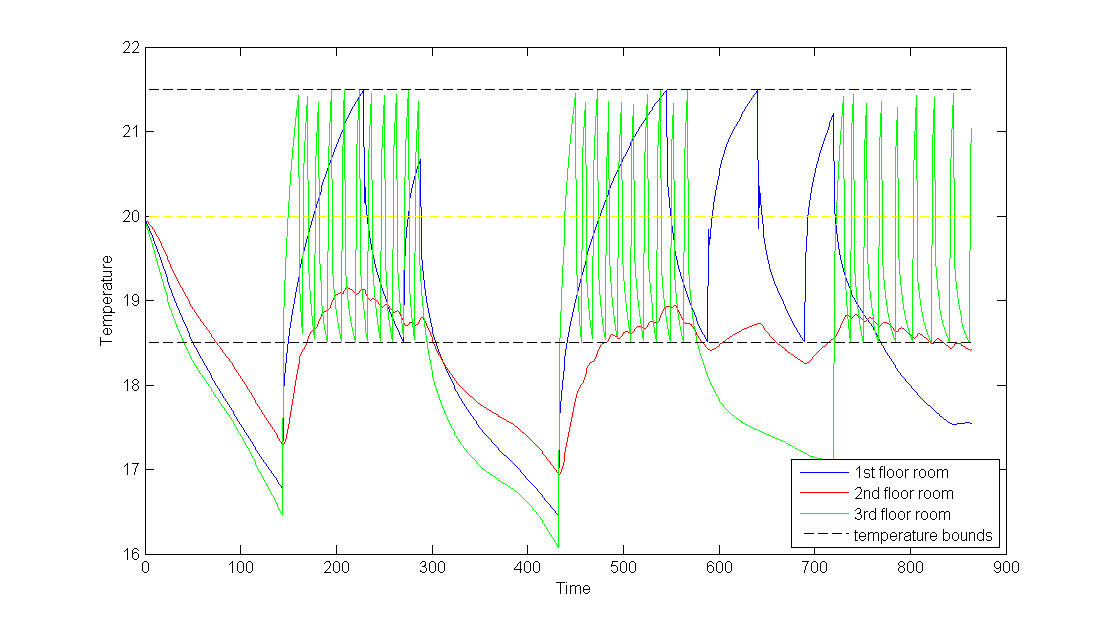
\includegraphics[width=0.45\textwidth, height=0.22\textwidth]{img/temperature_anal.png}
	\caption{\textit{Temperature of three rooms located one over the other having various customers along 6 days.}}
	\label{figTemper_onoff}
\end{figure}

%\section{Robotic application}


\section{State of the art}
%\subsection{Analysis of the market}
This analysis is performed in two important directions: the commercial and the research ones. In the commercial field, only 20\% of the hotel managers are used to looking for consistent demand statistics and use them actively for demand forecasting and profit management operations. The majority consider only the tourist information provided by specialized agencies instead of looking at past booking data to conclude on this. The existence of a software managing the whole bookings system is a common characteristic of many hotels. 

The algorithms existing in the market either in specialized softwares or open source solvers, over all those being used in Italy require the owner of the building to load the prices and priorities of the rooms for making its decisions. These softwares, however, tackle mostly the point of revenue management optimisation (offer campaigns and calculation of optimal room prices) but do not direct its resources in determining the optimal booking out of a given booking request situation. Until today, random assignments and first book - first take policies have been implemented in order to achieve not only a profit but also convenient client satisfaction.

If a few quantity of the software market is directed to optimising the booking, one can imply that even a smaller one attempts to optimize the objective from different perspectives. A smart agent in this sense would be an attractive proposal for optimising decreasing the energy consumption while maintaining the revenue at a maximum level. As commented afterwards, the problem of client satisfaction and personalized use forecasting while ensuring feasibility on the final solutions determines also an important developmental direction and a allows to generate an intelligent framework capable of deciding on the assignment based on a more objective complexity level \cite{grids}.

In the field of research, many works have attempted to manage the consumption of energy from a centralized point of view, in which small clients subscribe to a bigger entity in order to decrease the consumption by means of a closed communication mechanism \cite{central}. Domotics is an area dedicated to the automation of environments and to the increasing of their receptiveness to human beings in order to perform tasks more optimally. One of the most salient topics in the present has been that of providing different frameworks with the awareness of energy consumption and with it generate even communication patterns that ensure optimality in request reception (e.g. turn off the lights and turn them on again)\cite{web}.

A framework like the one proposed in this work would therefore:
\begin{enumerate}
	\item Represent a good opportunity to compete against softwares using other decision techniques.
	\item Ensure the capacity of solving multi objective problems.
	\item In both dimensions it implies improvements with respect to existing techniques
\end{enumerate}


%\subsection{Criteria used}
%???? %done
 
\section{Previous heat and control analysis}
In order to analyse the heat fluxes governing the heat transmission of a building there are two ways to proceed: taking blueprints of the building and, knowing all the material properties, making a heat analysis of every room, or taking the temperature of every room and identify the parameters to know the behave of heat fluxes. Because both approaches lead to the solution, we decided to make two independent previous analysis. \\
Each procedure is based on the equivalence having on the left side the summation of heat fluxes at a specific time instant and on the right side the variation of the internal energy from an instant to the following one:
$$q_{tot_{t}} = \Sigma q_{k_{t}} + \Sigma q_{h_{t}} + \Sigma q_{vent_{t}} + \Sigma q_{sun_{t}} + q_{pump_{t}}$$
$$q_{tot_{t}} = \rho V c_{p} \frac{d T}{d t}$$
Where:

$q_{k}$ is the thermal convection; \\
$q_{h}$ is the thermal conduction; \\
$q_{vent}$ is the ventilation flux according to the norm UNI/TS 11300; \\
$q_{sun}$ is the sun radiation took from weather forecast; \\
$q_{pump}$ is the heat flux coming from the heat pump (if activated); \\
$\rho V c_{p} \frac{d T}{d t}$ is the time derivative of the internal energy.

\subsection{Blueprint analysis strategy}
Since the used scenarios must be realistic we planned three kind of room according with their price and structure ($25$ $m^2$, $50$ $m^2$, $75$ $m^2$) and the same amount of customer kinds.
Every wall is made by common bricks (density: $2000$ $\frac{kg}{m^3}$; heat capacity: $0.9$ $\frac{kJ}{kg K}$; thermal conduction: $8 e^{-4}$ $\frac{kJ}{s m K}$); the exterior wall thickness is $0.4$ $m$, while the interior one is $0.1$ $m$. Every room have at least a window and one door on the corridor. The windows are made by common glass (density: $2400$ $\frac{kg}{m^3}$; heat capacity: $0.84$ $\frac{kJ}{kg K}$; thermal conduction: $9.6 e^{-4}$ $\frac{kJ}{s m K}$), and its thickness is $0.04$ $m$, while the doors are assumed to be like the interior wall for their heat behaviour. To run these initial set of experiments we decided to use real heat pumps (any other kind of heat source do not change the result) taken by the commercial catalogue Daikin Industries, in particular we used the heat pump called 'FTXZ35N'.

Due to the fact computer cannot handle continuous domain, the heat transfer equation must be discrete:
$$q_{tot_{t}} = \rho V c_{p} \frac{d T}{d t} \hspace{5mm} --> \hspace{5mm} \frac{q_{tot_{t}}}{\rho V c_{p}} = \frac{T_{t+1} - T_{t}}{time \\ gap}$$
Then, we can rewrite the equation:
$$K_{i,j} (T_{i,t} - T_{j,t}) = \frac{C_{i}}{time \\ gap} (T_{i,t+1} - T_{i,t})$$
Where:

$K_{i,j}$ is the heat transfer coefficient from the room j to i; \\
$C_{i,j}$ is the capacitance of the room i;

\subsection{System identification strategy}
The practise requires the temperature of the air of each room at each instant of the analysis   



E-plus

bla bla

\subsection{P control vs. ON/OFF control}


map of the hotel

different curves for the temperature depending on floors

gap-time

Assumptions on the hotel (temperature in - out, sun)




\section{analysis of the problem}
 
maximize revenue

minimize costs

reject request

Optimized software used is Gurobi

?formulas?

\input{results.tex}

\section{Conclusion}



%The robot used to collect the data is a Lego NXT robot equipped with a sensor developed at ECN. This robot is classified as a unicycle robot (2,0). The sensor bar is made of eight binary Reed sensors, which detects magnetic field. The detectors are spaced by 1 cm. The strip of sensors is located so that it is perpendicular to the x-axis of the robot, at a known position along $\textrm{X}_m$.
%The magnets are the beacons of the localization system. They are arranged as a squared array with a spacing of 55 mm.
%
%The robot also has two encoders, with a resolution of 360 dots per revolution.
%
%The localization system uses an EKF (Extended Kalman Filter).
%
%\section{First Lab}

In this first lab session, the use of extended Kalman filter for path estimation has been investigated. The complete Matlab files are provided in the folder \texttt{src/part1}.

\subsection{Discrete Evolution Model}\label{secDiscreteModel}

The model of the robot in continuous time can be expressed as\footnote{The value of $2L$ corresponds to the distance between the fixed wheels, represented in the Matlab files by the variable \texttt{trackGauge}.}:
$$\left[\begin{array}{c}
\dot{x} \\ \dot{y} \\ \dot{\theta}
\end{array}\right] =
\left[\begin{array}{c}
V\cos\theta \\ V\sin\theta \\ \omega
\end{array}\right]
\qquad\qquad
\left[\begin{array}{c}
V \\ \omega
\end{array}\right] =
\left[\begin{array}{cc}
\frac{r}{2} & \frac{r}{2} \\ \frac{r}{2L} & -\frac{r}{2L}
\end{array}\right] 
\left[\begin{array}{c}
\dot{q}_R \\ \dot{q}_L
\end{array}\right]
$$

Through a forward Euler discretization we can obtain the following:
$$\left[\begin{array}{c}
x_{k+1} \\ y_{k+1} \\ \theta_{k+1}
\end{array}\right] =
\left[\begin{array}{c}
x_k + U_{1,k}\cos\theta_k \\ y_k + U_{1,k}\sin\theta_k \\ \theta_k + U_{2,k}
\end{array}\right]
\qquad\qquad
\left[\begin{array}{c}
U_{1,k} \\ U_{2,k}
\end{array}\right] =
\left[\begin{array}{cc}
\frac{r}{2} & \frac{r}{2} \\ \frac{r}{2L} & -\frac{r}{2L}
\end{array}\right] 
\left[\begin{array}{c}
\Delta q_{R,k} \\ \Delta q_{L,k}
\end{array}\right]
$$
where $\Delta q_{R,k}$ represents the angle spanned by the right wheel within the time interval $\Delta t$ (i.e. $\Delta q_{R,k}=q_{R,k+1}-q_{R,k}$); the same works for $\Delta q_{L,k}$.

We implemented the model in the Matlab file called \texttt{EvolutionModel.m}, and we changed the script \texttt{ShowOdometry.m} so that it uses both our model and the default one (that has been renamed as \texttt{EvolutionModelDefault.p}). The correctness of our results is monitored by a matrix called \texttt{errX}, whose columns are defined as the difference given by the evolution of the new state obtained using the original \texttt{EvolutionModelDefault.p} and the state returned by our function. After the main loop of the script \texttt{ShowOdometry.m}, the error components are plotted in a figure. As expected, the result is that all the values are exactly zero, meaning that the model has been properly implemented.

Before proceeding, we had a look at the Cartesian speed of the robot. As shown in figure \ref{figSpeed} the estimation has some persistent oscillations. This is due to the not infinite resolution of the encoders, that introduce an error. The real linear speed is likely around $55\,\textrm{mm/s}$, while the angular one could be nearly zero.

\begin{figure}
	\centering
	\includegraphics[width=0.4\textwidth]{img/part1/odomVel.pdf}
	\caption{linear and angular speed estimated by odometry on the track \texttt{line1magnet}.}
	\label{figSpeed}
\end{figure}



\subsection{Extended Kalman Filter Equations}

The discrete time system that describes the evolution of robot's state has been already defined in the previous section:
$$\mathrm{X}_{k+1} =
\mathrm{X}_k + 
\begin{bmatrix} \cos\theta_k & 0\\ \sin\theta_k & 0\\ 0 & 1 \end{bmatrix}\mathrm{U}_k = 
f\left(\mathrm{X}_k, \mathrm{U}_k\right)
$$
In order to complete it, we need the following output equation:
$$ \mathrm{Y}_k =
\begin{bmatrix}
\cos\theta_k\left(x_m^\circ-x_k\right)+\sin\theta_k\left(y_m^\circ-y_k\right)\\
\cos\theta_k\left(y_m^\circ-y_k\right)-\sin\theta_k\left(x_m^\circ-x_k\right)
\end{bmatrix} =
g\left(\mathrm{X}_k\right)
$$
Where $\mathrm{Y}_k$ corresponds to the components of the distance between the detected magnet and the robot's origin (projected in robot's reference frame).

Since the system is not linear, the standard Kalman filter cannot be used; instead, we can evaluate the linear approximation of this system and estimate the path through an extended Kalman filter. The matrices that we need are the following:
\begin{flalign*}
A &= \frac{\partial f\left(\mathrm{X}_k, \mathrm{U}_k\right)}{\partial \mathrm{X}_k} = 
\begin{bmatrix}
1 & 0 & -U_{1,k}\sin\theta_k\\ 0 & 1 & U_{1,k}\cos\theta_k\\ 0 & 0 & 1
\end{bmatrix}
\\
B &= \frac{\partial f\left(\mathrm{X}_k, \mathrm{U}_k\right)}{\partial \mathrm{U}_k} =
\begin{bmatrix}
\cos\theta_k & 0 \\ \sin\theta_k & 0\\ 0 & 1
\end{bmatrix}
\\
C &= \frac{\partial g\left(\mathrm{X}_k\right)}{\partial \mathrm{X}_k} =
\begin{bmatrix}
-\cos\theta_k & -\sin\theta_k &
-\sin\theta_k\left(x_m^\circ-x_k\right)+\cos\theta_k\left(y_m^\circ-y_k\right)
\\
\sin\theta_k & -\cos\theta_k &
-\sin\theta_k\left(y_m^\circ-y_k\right)-\cos\theta_k\left(x_m^\circ-x_k\right)
\end{bmatrix}
\end{flalign*}






\subsection{Measurement Noise}

First of all, we set the covariance matrices all to zero. In such way, the estimation is assumed to be perfect, without noise.

In order to find the proper covariances, we reasoned about the factors that can corrupt the measurements. First of all, regarding the vertical component, i.e. \texttt{sigmaYmeasurement}, we assumed that a magnet could be located in any place between two sensors with uniform probability distribution, thus obtaining:
$$\sigma_{Ym} = \frac{\Delta Y}{\sqrt{12}} = \frac{10}{\sqrt{12}} $$
with $\Delta Y$ representing the spacing between two Reed receptors.

Regarding the value of \texttt{sigmaXmeasurement}, we considered two alternative methods for its calibration.

The first way is to set the scanning frequency to its maximum possible value (by setting \texttt{subSamplingFactor} to 1 in the file \texttt{RobotAndSensorDefinition.m}), make the robot follow a straight path (e.g. \texttt{line1magnet}) and check the region where a single magnet is detected more times consecutively. This allows to define an ``activation region'' for the sensors, namely $a_x$, that correspond to the interval where a sensor is able to detect the presence of a magnet. Referring to figure \ref{figHighSampling}, resulting from \texttt{line1magnet}, we found that a single magnet can be detected at most seven times.

\begin{figure}[htbp]
	\centering
	\hspace{\stretch{1}}
	\subfigure[Series of acquisitions from Reed sensors; each magnet is detected several times.\label{figHighSampling}]{\includegraphics[width=0.4\textwidth]{img/part1/samplingHighRate.pdf}}
	\hspace{\stretch{1}}
	\subfigure[Focus around a particular magnet. The activation region $a_x$ and the distance $d_x$ between two acquisitions are shown.\label{figHighSamplingZoom}]{\includegraphics[width=0.4\textwidth]{img/part1/samplingHighRateZoom.pdf}}
	\hspace{\stretch{1}}
	\caption{example of readings from the Reed sensors.}
\end{figure}

The distance between two consecutive scans is $d_x = 3\,\textrm{mm}$ (fig. \ref{figHighSamplingZoom}), and therefore we have that $a_x=18\textrm{mm}$. In addition, we must consider that the magnet could have activated the Reed sensors before the first measurement or after the last one. The estimated activation region has to be enlarged to $a_x+d_x=21\,\textrm{mm}$. We assumed that the magnet could be in any position of the activation region with the same probability, and therefore we could set \texttt{sigmaXmeasurement} to:
$$ \sigma_{Xm} = \frac{a_x+d_x}{\sqrt{12}} = \frac{21}{\sqrt{12}} $$

The previous method is based on the possibility of performing one test with a higher scanning sampling rate than the one normally used by the robot. Since this could be infeasible (because we simply cannot increase the sampling rate), a similar method to estimate measurement variance consists in repeating the same procedure with the standard sampling rate; in our case, we have to set \texttt{subSamplingFactor} to its original value, i.e. 4. Figure \ref{figLowSampling} shows the magnet detection in the test \texttt{diagonal45degrees}; due to the lower frequency, a magnet is detected at most 2 times, and therefore the values of $a_x$ and $d_x$ become the same: $12\,\textrm{mm}$ (fig. \ref{figLowSamplingZoom}). Therefore the position of a detected magnet can be, in the worst case, $12\,\textrm{mm}$ away from the activated Reed sensor. Assuming again a uniform probability distribution, it is possible to determine the standard deviation as:
$$ \sigma_{Xm} = \frac{a_x+d_x}{\sqrt{12}} = \frac{24}{\sqrt{12}} $$

\begin{figure}[htbp]
	\centering
	\hspace{\stretch{1}}
	\subfigure[Series of acquisitions from Reed sensors; each magnet is detected at most two times.\label{figLowSampling}]{\includegraphics[width=0.4\textwidth]{img/part1/samplingLowRate.pdf}}
	\hspace{\stretch{1}}
	\subfigure[Focus around a particular magnet. The activation region $a_x$ and the distance $d_x$ between two acquisitions here coincide.\label{figLowSamplingZoom}]{\includegraphics[width=0.4\textwidth]{img/part1/samplingLowRateZoom.pdf}}
	\hspace{\stretch{1}}
	\caption{example of readings from the Reed sensors.}
\end{figure}


%we guessed that any sensor can activate only within a \colorbox{pink}{restricted} area, $a_x$. In order to evaluate the length of this interval, we put the scanning frequency to the maximum possible (\texttt{subSamplingFactor = 1} in \texttt{RobotAndSensorDefinition.m}), and after one execution of \texttt{MagnetLoc.m} we obtained a the sequence of acquisitions shown in figure \ref{figMangetScanNoZoom}: one single magnet is detected several times, and therefore we can estimate the ``detectability range'' as the width of such sequence of readings (\ref{figMangetScanZoom}). We obtained $a_x=14\textrm{mm}$.
%
%\begin{figure}[htbp]
%	\centering
%	\hspace{\stretch{1}}
%	\subfigure[Series of acquisitions from Reed sensors; each magnet is detected several times.\label{figMangetScanNoZoom}]{\includegraphics[width=0.4\textwidth]{img/part1/figsamplinghigh.pdf}}
%	\hspace{\stretch{1}}
%	\subfigure[Focus around a particular magnet. The width $a_x$ is clearly shown and the additional uncertainty $f_x$ is reported referred to the case \texttt{subSamplingFactor=4}. \label{figMangetScanZoom}]{\includegraphics[width=0.4\textwidth]{img/part1/figsamplinghighzoom.pdf}}
%	\hspace{\stretch{1}}
%	\caption{example of readings from the Reed sensors.}
%\end{figure}
%
%In addition, there will be a further uncertainty coming from the readings frequency. One can imagine that, with an infinite frequency, the uncertainties will come from the value of $a_x$ only. However, since the readings have a finite frequency, the uncertainties will increase, and we can estimate them as the half of the distance between two sequential acquisitions. Once \texttt{subSamplingFactor} was reset to the initial value (i.e. 4), we found $f_x = 11\textrm{mm}$, that is the distance between two scans.

In conclusion, one can decides which method is more suitable. In general, the first one will be more precise, though not always feasible. Since it was possible to do so, we decided to set the value of \texttt{sigmaXmeasurement} to $\frac{21}{\sqrt{12}}$.



\subsection{Initial State Uncertainties}

Another parameter that has to be tuned is the variance of initial state. The error in the starting positioning is strictly related to user's imprecision in locating the robot in the proper location with the right orientation. We assumed that the positioning errors can be considered as Gaussian random variables with zero mean and standard deviations $\sigma_x = 5\,\textrm{mm}$, $\sigma_y = 5\,\textrm{mm}$ and $\sigma_\theta = 5^\circ$. With such values, initial errors will belong to the intervals $[-2\sigma,+2\sigma]$ with a probability of 95\%.





\subsection{Mahalanobis Threshold}

In order to choose a proper threshold for Mahalanobis distance, we used the Matlab function \texttt{chi2inv}, which has two parameters as input: the desired probability \texttt{P} of non-rejecting a good measure and the degrees of freedom \texttt{V} of our system. We used the two values \texttt{P=0.9} and \texttt{V=2} (\texttt{V} in this situation corresponds to the number of measurements that we have), thus obtaining the threshold $\sim\!4.6$.



\subsection{Tuning ``\texttt{sigmaWheels}''}\label{sectionSigmaWheel}

The last parameter that has to be tuned is \texttt{sigmaWheels}. To do so, we decided to run the program using the tracks named \texttt{oneloop} and \texttt{twoloops}; as criteria we chose the following:

\begin{enumerate}
	\item all the detected magnets must not be rejected;
	\item almost all neighbour magnets must be rejected;
	\item the initial and final position of the robot must be very similar.
\end{enumerate}

We used a dichotomic approach, starting from the value 1.0 as upper bound and 0 as lower bound. After some trials (some of them are shown in figure \ref{figSigmaTuning}; they have been performed on \texttt{twoloops}), the chosen value is \texttt{sigmaWheels = 0.1}, which ensures to reject the neighbours magnets and to keep the closest ones. In addition, initial and final positions are nearly equal (fig. \ref{figSigmaTuningPositions}).

\begin{figure}[htbp]
	\centering
	\hspace{\stretch{1}}
	\subfigure[$\sigma_W=1.0$]{\includegraphics[width=0.22\textwidth]{img/part1/mahaFail10.pdf}}
	\hspace{\stretch{1}}
	\subfigure[$\sigma_W=0.5$]{\includegraphics[width=0.22\textwidth]{img/part1/mahaFail05.pdf}}
	\hspace{\stretch{1}}
	\subfigure[$\sigma_W=0.2$]{\includegraphics[width=0.22\textwidth]{img/part1/mahaFail02.pdf}}
	\hspace{\stretch{1}}
	\subfigure[$\sigma_W=0.1$]{\includegraphics[width=0.22\textwidth]{img/part1/mahaFail01.pdf}}
	\hspace{\stretch{1}}
	\caption{tuning of $\sigma_W$ (\texttt{sigmaWheels}); the number of rejected neighbours magnet increases as $\sigma_W$ decreases. With $\sigma_W = 0.1$ we are able to reject all neighbours magnet while keeping the closest ones.}\label{figSigmaTuning}
\end{figure}

\begin{figure}[htbp]
	\centering
	\hspace{\stretch{1}}
	\subfigure[Track \texttt{oneloop}]{\includegraphics[width=0.22\textwidth]{img/part1/oneloop.pdf}}
	\hspace{\stretch{1}}
	\subfigure[Focus around initial an final positions]{\includegraphics[width=0.22\textwidth]{img/part1/oneloopFocus.pdf}}
	\hspace{\stretch{1}}
	\subfigure[Track \texttt{twoloops}]{\includegraphics[width=0.22\textwidth]{img/part1/twoloops.pdf}}
	\hspace{\stretch{1}}
	\subfigure[Focus around initial an final positions]{\includegraphics[width=0.22\textwidth]{img/part1/twoloopsFocus.pdf}}
	\hspace{\stretch{1}}
	\caption{estimated paths (odometry and KF) in the two tracks \texttt{oneloop} and \texttt{twoloops}. In both cases, the distance from initial to final position is around $3\,\textrm{mm}$, that could be due to human driver's imprecisions}\label{figSigmaTuningPositions}
\end{figure}

Finally, we tested this set of parameters with the other tracks, obtaining for all of them good estimations.

%
%\newpage
%
%\section{First Lab}

In this first lab session, the use of extended Kalman filter for path estimation has been investigated. The complete Matlab files are provided in the folder \texttt{src/part1}.

\subsection{Discrete Evolution Model}\label{secDiscreteModel}
%
\end{document}